\RequirePackage[l2tabu, orthodox]{nag}
%\pdfminorversion=4
\documentclass[a0paper,portrait,fontscale=0.35]{baposter}

\usepackage{amsfonts,amsmath,amsthm,amssymb,commath}
\usepackage{graphicx,subcaption}
\usepackage[most,skins,theorems]{tcolorbox}
\usepackage{color}

\usepackage{relsize}
\usepackage{natbib}
\usepackage{microtype}

\usepackage{tikz}
\usetikzlibrary{decorations.pathreplacing}

\newcommand{\PSF}{\text{PSF}}
\newcommand{\argmin}{\text{argmin}}

%%% Define a caption font
\newcommand{\mycaption}[1]{
  {
    \smaller
    \emph{#1}
  }
}

\theoremstyle{plain}
\newtheorem{thm}{\protect\theoremname}
  \theoremstyle{plain}
  \newtheorem{lem}[thm]{\protect\lemmaname}
  \theoremstyle{definition}
  \newtheorem{defn}[thm]{\protect\definitionname}
  \theoremstyle{plain}
  \newtheorem{prop}[thm]{\protect\propositionname}
  \theoremstyle{definition}
  \newtheorem{example}[thm]{\protect\examplename}

%%% Color Definitions %%%%%%%%%%%%%%%%%%%%%%%%%%%%%%%%%%%%%%%%%%%%%%%%%%%%%%%%%
%\definecolor{oxford_blue}{RGB}{14,31,71}
%\definecolor{oxford_border}{RGB}{14,31,71}

%\definecolor{cambridge_blue}{RGB}{64,76,0}
%\definecolor{cambridge_blue}{RGB}{163, 193, 173}
%\definecolor{cambridge_border}{RGB}{163, 193, 173}

\definecolor{cambridge_blue}{RGB}{49,72,56}
\definecolor{cambridge_border}{RGB}{49,72,56}

\tcbset{highlight math style={enhanced, 
    colframe=cambridge_blue, colback=white}}

\begin{document}
\typeout{Poster rendering started}

\begin{poster}
{
    % Show grid to help with alignment
    grid=false,
    columns=6,
    % Column spacing
    colspacing=0.7em,
    % Color style
    %headerColorOne=cyan!20!white!90!black,
    %borderColor=cyan!30!white!90!black,
    headerColorOne=cambridge_blue,
    borderColor=cambridge_border,
    headerFontColor=white,
    % Format of textbox
    textborder=faded,
    % Format of text header
    headerborder=open,
    headershape=smallrounded,
    headershade=plain,
    background=none,
    bgColorOne=cyan!10!white,
    %headerheight=0.11\textheight,
    headerheight=0.095\textheight,
    eyecatcher=false,
}
% Eye Catcher: Oxford logo and personal picture
{
%  \makebox[0.23\textwidth]{
%    \begin{tabular}{cc}
%    
\includegraphics[height=0.055\textheight]{./img/InFoMM}
%      &
%    %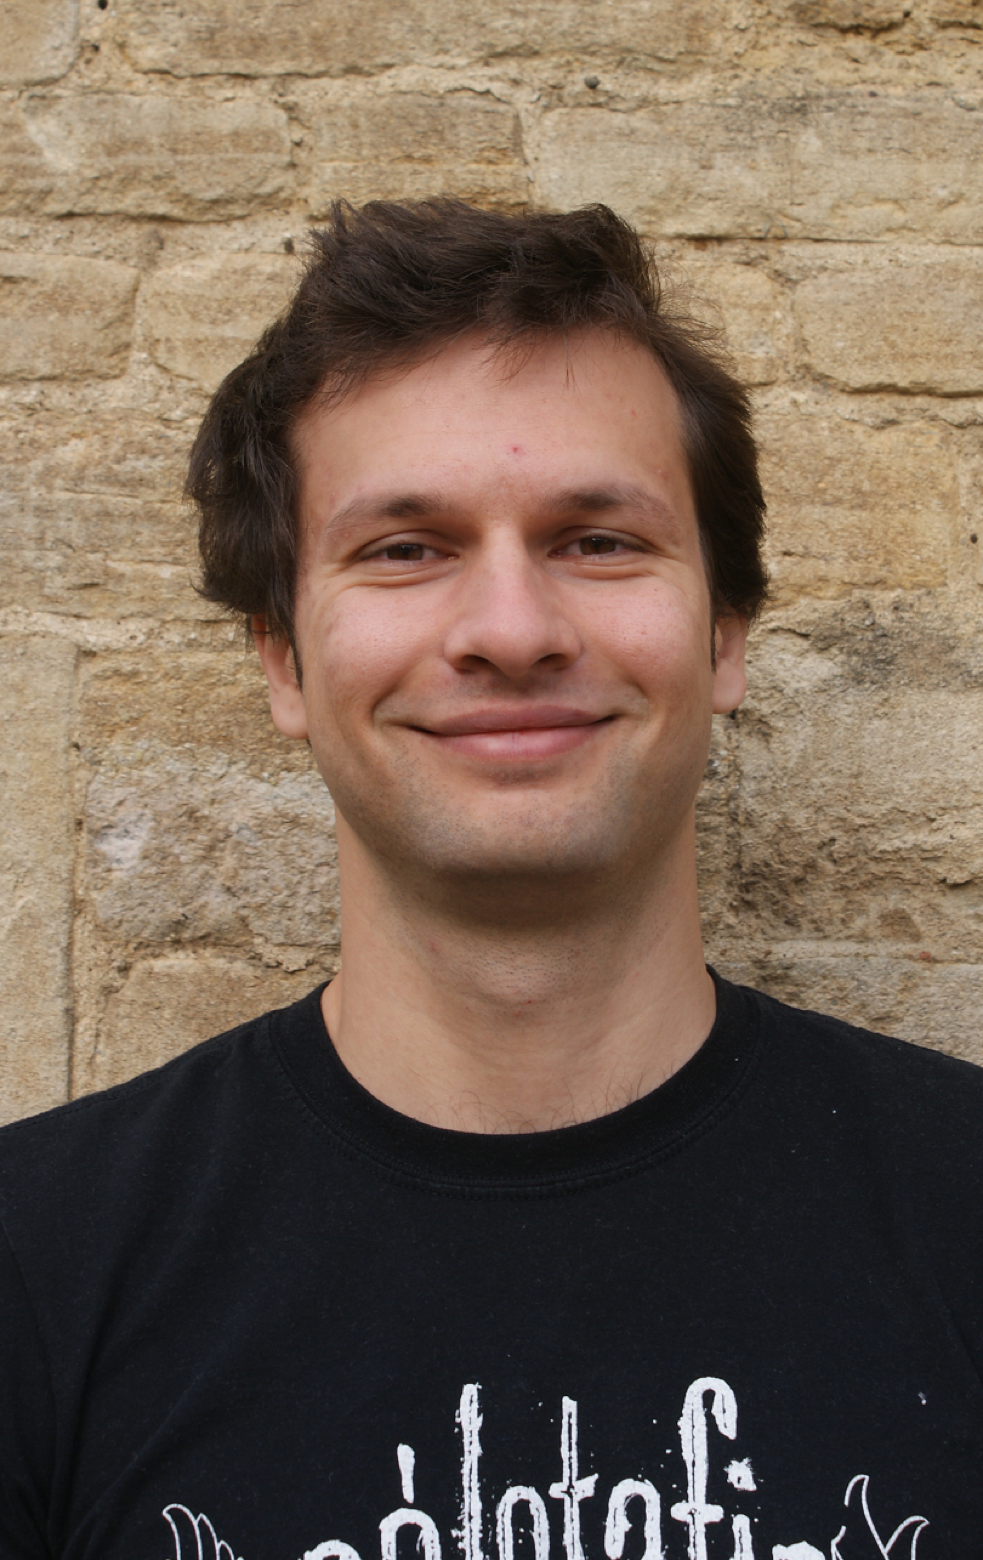
\includegraphics[height=0.10\textheight]{./img/me}
%    \end{tabular}
%    \hfill
%  }
}
%%% Title %%%%%%%%%%%%%%%%%%%%%%%%%%%%%%%%%%%%%%%%%%%%%%%%%%%%%%%%%%%%%%%%%%%%%
{
  %%\textsc{Source Reconstruction \vspace{0.2cm}\\From Hydrophone Data}
  \textsc{Spatially Variable Deconvolution\vspace{0.2cm}\\ 
    for Lightsheet Microscopy\vspace{0.2em}}
  \vspace{0.3em}
}
%%% Authors %%%%%%%%%%%%%%%%%%%%%%%%%%%%%%%%%%%%%%%%%%%%%%%%%%%%%%%%%%%%%%%%%%%
{
  \vspace{0.1em}
  \hspace{-0.65em}
  {
    \underline{\textbf{Bogdan Toader}}\textsuperscript{1},
    \textbf{TODO update St\'{e}phane Chr\'{e}tien}\textsuperscript{2}, 
    \textbf{Andrew Thompson}\textsuperscript{3}
  } \\[0.2em]
  {
    \textsuperscript{1}University of Cambridge,
    \textsuperscript{2}University of Lyon 2, 
    \textsuperscript{3}National Physical Laboratory
  }
}
%%% InFoMM Logo %%%%%%%%%%%%%%%%%%%%%%%%%%%%%%%%%%%%%%%%%%%%%%%%%%%%%%%%%%%%%%%
%{
%  %\makebox[0.23\textwidth]{
%  \makebox[0.32\textwidth]{
%    \hfill
%    \begin{tabular}{ccc}
%    %
\includegraphics[height=0.055\textheight]{./img/InFoMM}
%      
\includegraphics[height=0.04\textheight]{./img/InFoMM}
%      &
%    %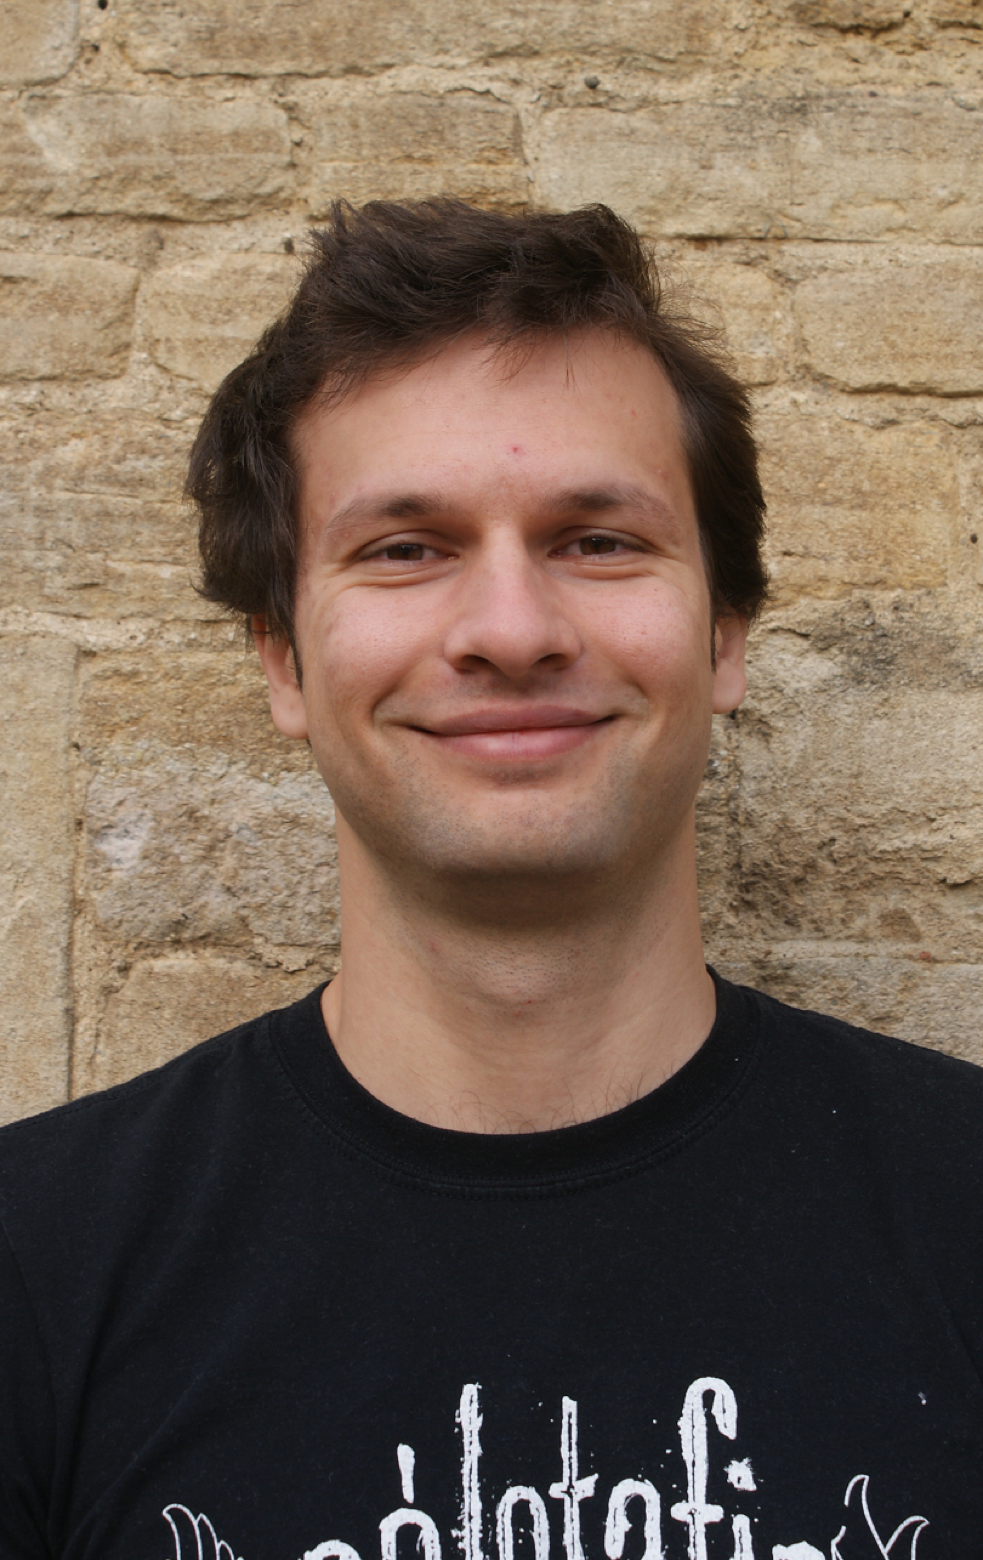
\includegraphics[height=0.10\textheight]{./img/me}
%      
\includegraphics[height=0.04\textheight]{./img/oxlogo}
%      \\
%      
\includegraphics[height=0.04\textheight]{./img/turinglogo2}
%      &
%      
\includegraphics[height=0.04\textheight]{./img/edinlogo}
%      %&
%      %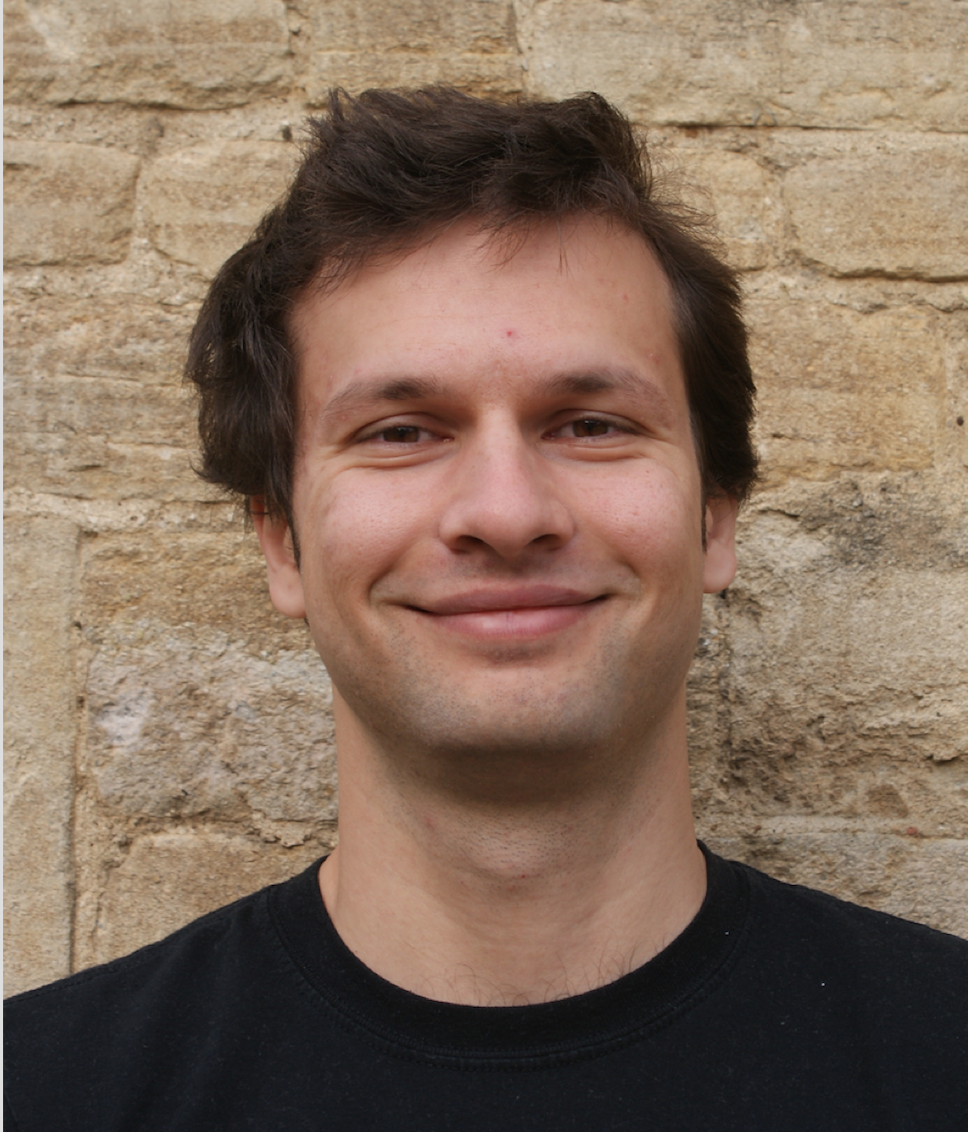
\includegraphics[height=0.05\textheight]{./img/me_square}
%    \end{tabular}
%  }
%  %}
%}
{
  %\makebox[0.23\textwidth]{
  \makebox[0.32\textwidth]{
    \hfill
    \begin{tabular}{ccc}
      
\includegraphics[height=0.04\textheight]{./img/camlogo}
    \end{tabular}
  }
  %}
}
\headerbox{lightsheet microscopy}{name=lightsheet, span=3, column=0, row=0}{

  \begin{minipage}[t]{\textwidth}
    TODO: a few words about why lightsheet is good

    Light sheet microscopy is a type of fluorescence microscopy used in cell biology due to its fast acquisition times and low photo-damage to the sample. This is achieved by selectively illuminating a slice of the sample using a sheet of light and detecting the emitted fluorescence signal using a dedicated objective orthogonal to the plane of the sheet. 

    %Consequently, the effective point spread function (PSF) of the microscope is space varying, which adds an additional layer of complexity to the problem of deconvolution of such images.
     \begin{itemize} 
      \item
        Project aim: computationally improve the 
        quality of light sheet microscopy images.
    \end{itemize}

  \end{minipage}
  \vspace{1pt}
    
  \begin{minipage}[t]{\textwidth}
    \begin{minipage}[t]{0.48\textwidth}
      \begin{center}
        \larger
        {\color{blue}\textbf{\textsc{Light-sheet microscope}}}\\
        %\textit{$x$ is the discrete measure\\
        %we want to reconstruct.}
      \end{center}
          
      \begin{minipage}[t]{\textwidth}
        \centering
        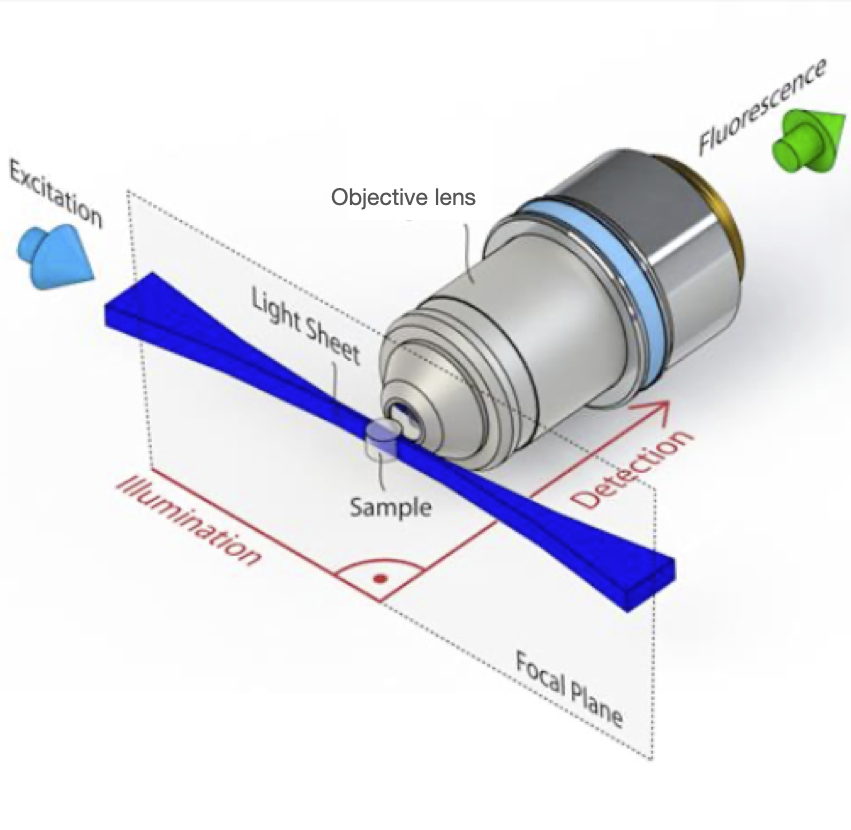
\includegraphics[width=0.8\textwidth]{img/spim.png}
       
        \mycaption{Figure credit: J\"{o}rg Ritter, PhD thesis (2011)}
        %\mycaption{The input signal is a sum of Diracs \\ represented 
         % as a discrete measure.}
      \end{minipage}
     
      %\vspace{-0.5em}
      %\begin{center}
      %  \tcbhighmath[colback=blue!10!white, frame hidden]{
      %    x(t) = \sum_{i=1}^{k} a_i \cdot \delta_{t_i},
      %    %\quad a_i > 0
      %  }
      %\end{center}

      \hspace{1em}
      %{ \smaller 
      %  $t_i$ and $a_i$ ($i=1,\ldots,k$) are the locations\\
      %  and magnitudes of the point sources.}
      
      A light-sheet microscope consists of two objectives: TODO etc
    
    \end{minipage}
    %
    \begin{minipage}[t]{0.48\textwidth}
      \begin{center}
        \larger
        {\color{blue}\textbf{\textsc{Spatially varying PSF}}}\\
        %\textit{$y_i$ are the samples\\
        %  we use to reconstruct $x$.}
      \end{center}
      
      \begin{minipage}[t]{\textwidth}
        \centering
        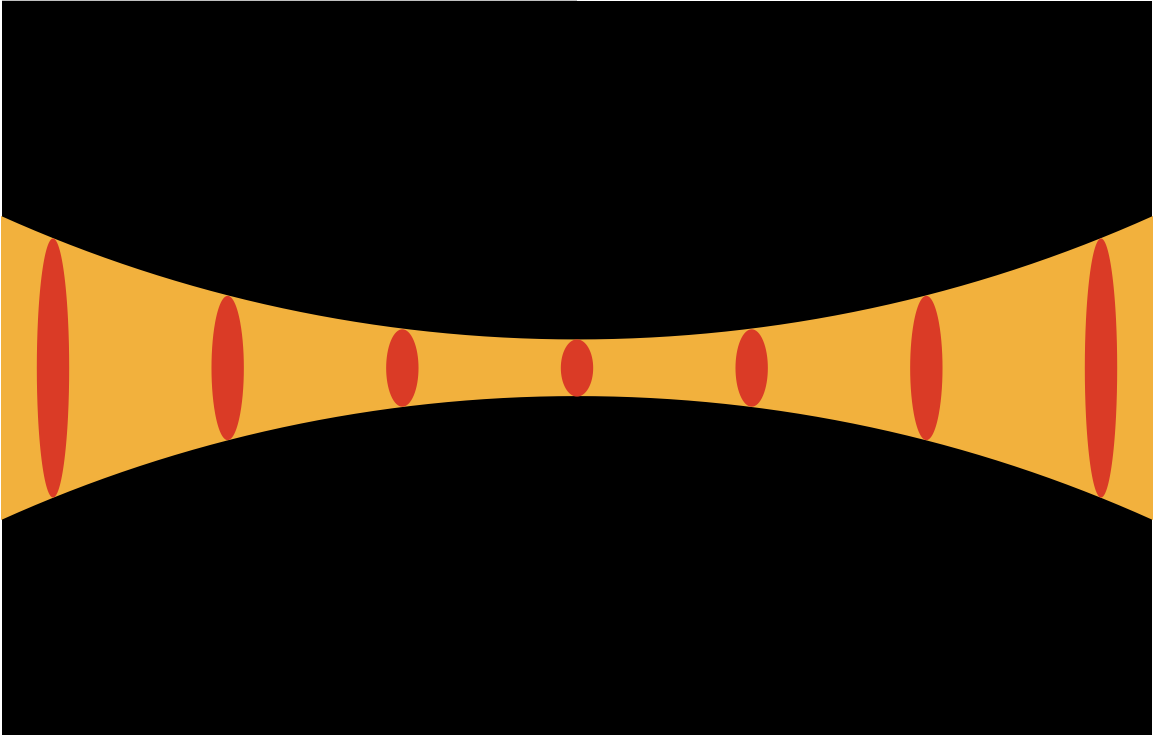
\includegraphics[width=0.8\textwidth]{img/psf_4.png}

        %\mycaption{The measured signal is the convolution of the \\ input signal
        %  with a window function $\psi$.}
      \end{minipage}

      \begin{center}
        \larger
        {\color{red}\textbf{\textsc{Problem}}}\\
      \end{center}
      \vspace{-0.5em}
      \begin{tcolorbox}[colback=red!10!white,colframe=red]
        Due to the combination of light-sheet and the objective PSF, 
        the effective PSF of the system is spatially varying, and
        therefore standard deconvolution approaches are not applicable.
      \end{tcolorbox}

    \end{minipage}
  \end{minipage}
}
\headerbox{psf model}{name=model, span=3, column=3, row=0}{

  \begin{minipage}[t]{\textwidth}
    TODO
    We calculate the objective PSF $h$ by using a model 
    that includes defocus etc etc. TODO: reference to paper 
    \begin{tcolorbox}[colback=teal!10!white,colframe=white]
      \begin{equation}
        h(x,y,z) = \left|
          \iint g_{\sigma} * p(\kappa_x,\kappa_y) e^{
            2 i \pi z 
            \sqrt{(n/\lambda)^2 - \kappa_x^2 - \kappa_y^2}
          }
          e^{
            2 i \pi (\kappa_x x + \kappa_y y)
          }
          \dif \kappa_x \dif \kappa_y
        \right|^2
        \label{eq:psf model}
      \end{equation}
    \end{tcolorbox}
    with the pupil function $p$ defined 
    \begin{tcolorbox}[colback=teal!10!white,colframe=white]
      \begin{equation}
        p(\kappa_x,\kappa_y) = \begin{cases}
          e^{2i\pi \sum_{j=1}^{15} c_i Z_j(\kappa_x,\kappa_y)}
          \quad
            &\text{for} \quad
            \rho = \sqrt{\kappa_x^2 + \kappa_y^2} \leq NA/\lambda,\\
            0, \quad &\text{otherwise.}
        \end{cases}
      \end{equation}
    \end{tcolorbox}
    where the phase of the pupil function is computed by least-squares
    fitting of the coefficients of the first $15$ Zernike polynomials
    using an image of a bead.
  \end{minipage}

  \vspace{10pt}
  \begin{minipage}[t]{\textwidth}
    \begin{minipage}[t]{0.38\textwidth}
      The parameters of the model are given by
      the experimental setup used to acquire the image:
      \begin{itemize}
        \item $n$ - refractive index
        \item $\lambda$ - wave length
        \item NA - numerical aperture
        \item $g_{\sigma}$ Gaussian blur to take into account
          other properties not accounted for in our model
      \end{itemize}
    \end{minipage}
    %
    \begin{minipage}[t]{0.3\textwidth}
      \centering
      \raisebox{\dimexpr-\height+\ht\strutbox}{
        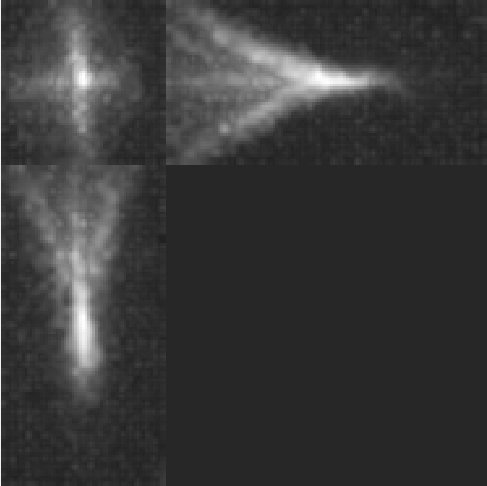
\includegraphics[height=0.1\textheight]{img/psf_bead.png}
      }

      \vspace{0.3em}
      \mycaption{
        Bead image (MIP)
      }
    \end{minipage}
    %
    \begin{minipage}[t]{0.3\textwidth}
      \centering
      \raisebox{\dimexpr-\height+\ht\strutbox}{
        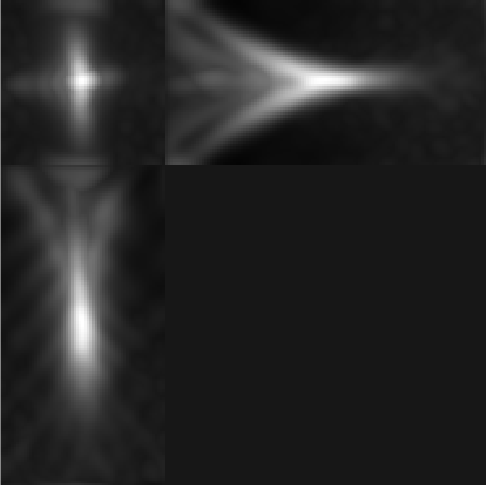
\includegraphics[height=0.1\textheight]{img/psf_zernike_sigma.png}
      }

      \vspace{0.3em}
      \mycaption{
        Estimated objective PSF (MIP)
      }
    \end{minipage}
  \end{minipage} 
}

\headerbox{image formation model}{name=psf, span=3, column=0, below=lightsheet}{
  \begin{minipage}[t]{\textwidth} 
    \begin{center}
      \larger
      \textbf{\textsc{Forward model}}
    \end{center}

    The sample $s$ illuminated at $z=z_0$ by the light-sheet $l$
    and the photons are collected by an objective with PSF $h$:
    \begin{center}
      \tcbhighmath[colback=red!10!white, frame hidden]{
        f(x,y,z_0) = \iiint l_{avg_y}(u,v,w) s(u,v,w - z_0) h(x-u,y-v,w) \dif u \dif v \dif w
        \label{eq:lightsheet model}
      }
    \end{center}
    where $h$ is given in \eqref{eq:psf model} 
    and $l$ is calculated similarly (TODO explain)

    TODO: insert diagram of the image formation to explain the forward model

  \end{minipage}
}

\headerbox{Results -- simulated data}{name=resultssim, span=3, column=3, below=lightsheet}{
    \begin{center}
      \larger
      \textbf{\textsc{Reconstruction}}
    \end{center}

    TODO: refine this text, also make it take into account that
    we don't always use L2 for fidelity or TV for regularization.
    Let $\hat{f}$ be the image data and
    $f(s)$ the result of applying the forward
    model to the sample $s$.

    To recover $s$, we solve:
    \begin{center}
      \tcbhighmath[colback=red!10!white, frame hidden]{
        \text{Find }
        \hat{s} \in 
        \argmin_{s} \left\{
          \| \hat{f} - f(s)   \|_{L_2}
          + \lambda TV(s)  
        \right\}
      }
    \end{center}
    using a version of the Primal Dual Hybrid Gradient (PDHG) 
    algorithm. TODO: reference.

    TODO: insert results. Then in the real data section, say the
    results are obtained by solving the same optimization problem.

}

\headerbox{Results -- real data}
{name=resultsreal,column=0, below=psf, span=6}{
  \begin{minipage}[t]{0.51\textwidth} 
    \begin{center}
      \larger
      \textbf{\textsc{Beads}}
    \end{center}

    Full resolution image: 1127 x 111 x 100

    \begin{minipage}[t]{\textwidth}
      \centering
      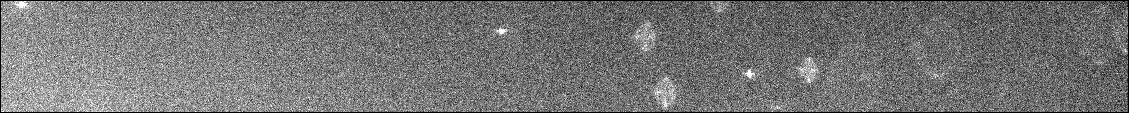
\includegraphics[width=0.5\textwidth]{img/fBeads_xy1.png}
      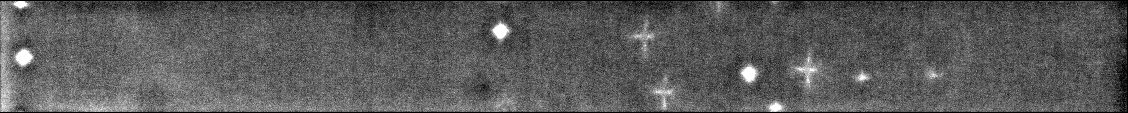
\includegraphics[width=0.5\textwidth]{img/urecBeads_h_xy1.png}
      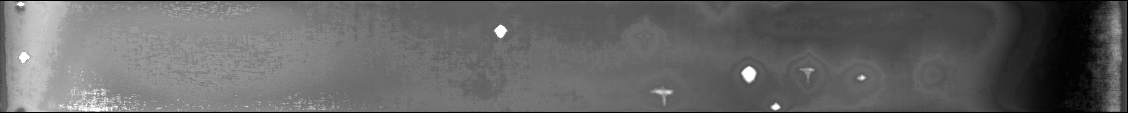
\includegraphics[width=0.5\textwidth]{img/urecBeads_xy1.png}
    \end{minipage}

    \begin{center}
      \mycaption{
        Data (top), constant PSF deconvolution (middle),
        model deconvolution (bottom)
      }
    \end{center}

    \begin{minipage}[t]{\textwidth}
      %\hspace{0.6cm}
      \centering
      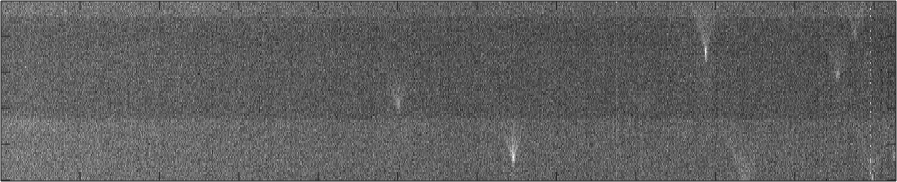
\includegraphics[width=0.5\textwidth]{img/fBeads_xz1.png}
      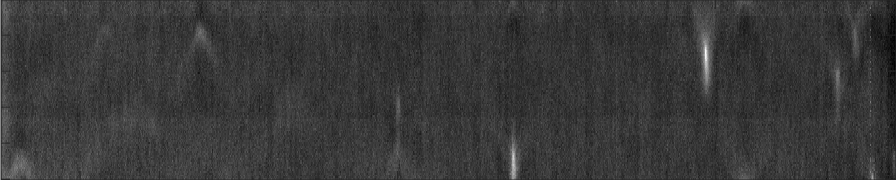
\includegraphics[width=0.5\textwidth]{img/urecBeads_h_xz1.png}
      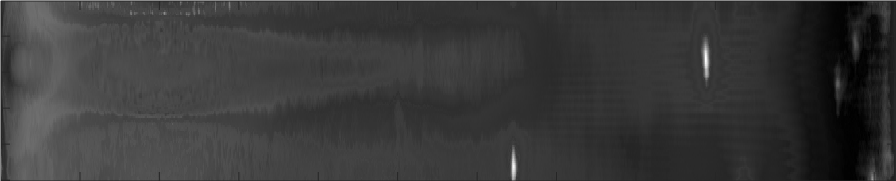
\includegraphics[width=0.5\textwidth]{img/urecBeads_xz1.png}
    \end{minipage}

    \begin{center}
      \mycaption{
        Data (top), constant PSF deconvolution (middle),
        model deconvolution (bottom)
      }
    \end{center}


%    \vspace{-1em}
%    \begin{minipage}[h]{0.5\textwidth}
%      \begin{itemize}
%        \item \textbf{Exact measurements:} 
%          the level method finds the correct
%          locations of the point sources with high
%          accuracy -- see the localisation error
%          for two sources as the distance between them
%          goes to zero in the bottom left figure. 
%        \item \textbf{Noisy measurements:}
%          As the distance between two sources
%          decreases, they are replaced with one source
%          with higher intensity in the reconstructed
%          signal.
%      \end{itemize}
%    \end{minipage}
%    %
%    \begin{minipage}[h]{0.49\textwidth}
%      \centering
%      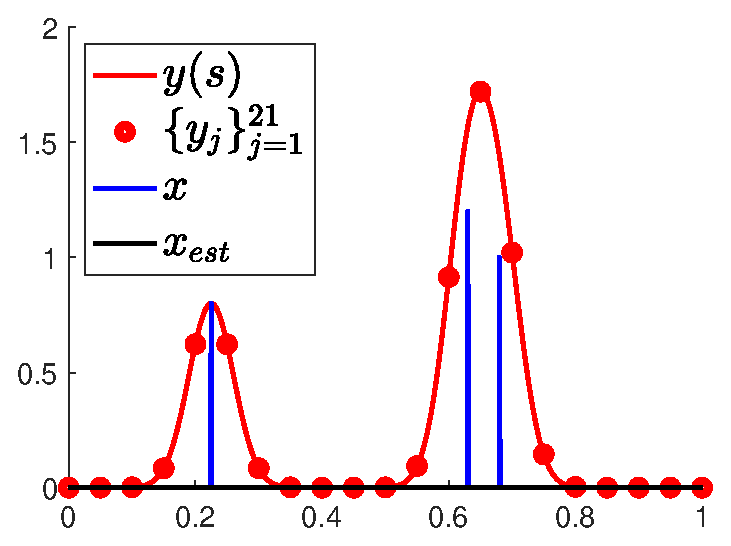
\includegraphics[height=0.1\textheight]{img/1d_base.eps}
%      %\vspace{-0.5em}
%      
%      \mycaption{Example of setup with noise-free\\ 
%        measurements, solved to accuracy $10^{-6}$.}
%    \end{minipage}
% 
%    \vspace{0.5em}
%    \begin{minipage}[h]{0.97\textwidth}
%      \begin{minipage}[h]{0.5\textwidth}
%        \centering
%        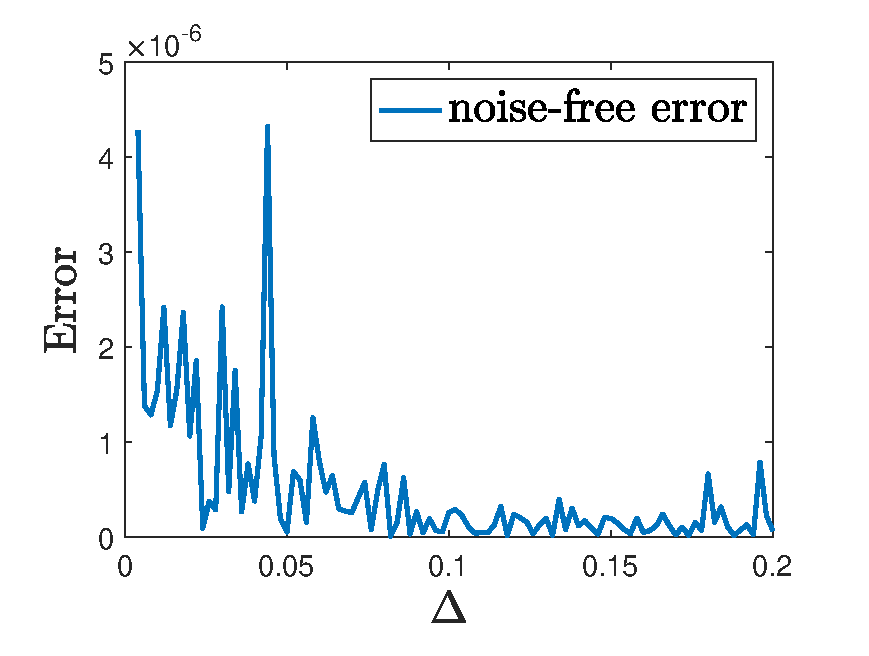
\includegraphics[height=0.12\textheight]{img/1d_error_noisefree.eps}
%        %\vspace{-0.5em}
%      \end{minipage}
%      %
%      \begin{minipage}[h]{0.5\textwidth}
%        \centering
%        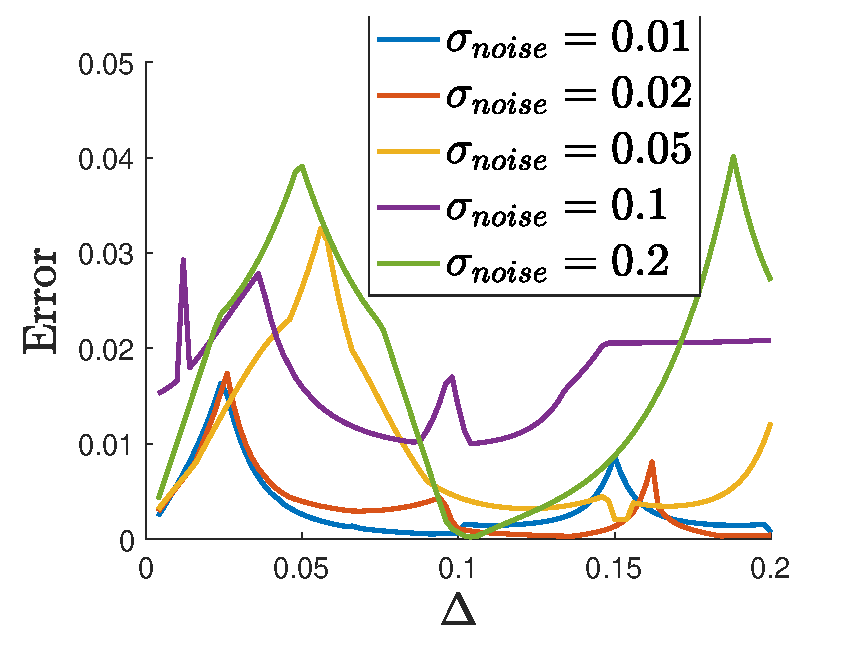
\includegraphics[height=0.12\textheight]{img/1d_error_noisy.eps}
%        %\vspace{-0.5em}
%      \end{minipage}
%
%      \vspace{-1em}
%      \begin{center}
%        \mycaption{Localisation error for two point sources
%          as the distance $\Delta$ between them increases 
%          from $0.004$ to $0.2$ in the noise-free case (left)
%          and noisy case for Gaussian noise with standard deviation
%          $0.01$, $0.02$, $0.05$, $0.1$, $0.2$ (right).
%          The convolution kernel
%          is Gaussian with $\sigma=0.05$, intensities are $1$ 
%          and $m=21$ equispaced samples.
%        }
%        \end{center}
%    \end{minipage}
  \end{minipage}
  %
  \begin{minipage}[t]{0.48\textwidth}
    \begin{center}
      \larger
      \textbf{\textsc{Marchantia}}
    \end{center}

    TODO: include the latest results here because better

    Full resolution image: 1127 x 155 x 100

    \begin{minipage}[t]{\textwidth}
      %\hspace{0.6cm}
      \centering
      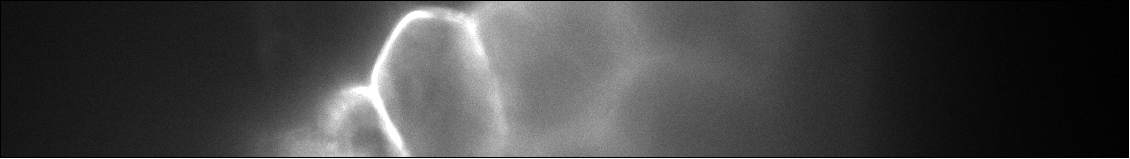
\includegraphics[width=0.5\textwidth]{img/f_xy1.png}
      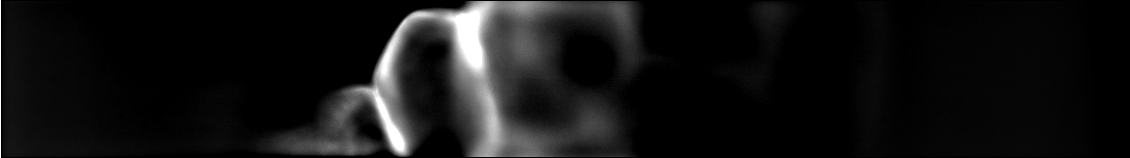
\includegraphics[width=0.5\textwidth]{img/urec_h_xy1.png}
      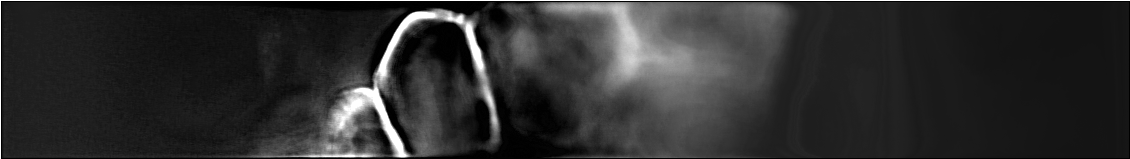
\includegraphics[width=0.5\textwidth]{img/urec_xy1.png}
    \end{minipage}

    \begin{center}
      \mycaption{
        Data (top), constant PSF deconvolution (middle),
        model deconvolution (bottom)
      }
    \end{center}

    \begin{minipage}[t]{\textwidth}
      %\hspace{0.6cm}
      \centering
      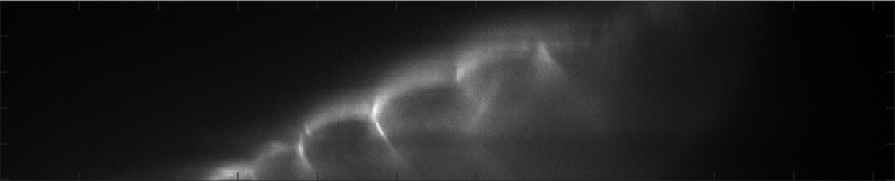
\includegraphics[width=0.5\textwidth]{img/f_xz1.png}
      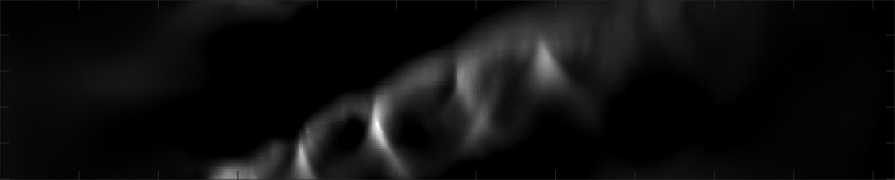
\includegraphics[width=0.5\textwidth]{img/urec_h_xz1.png}
      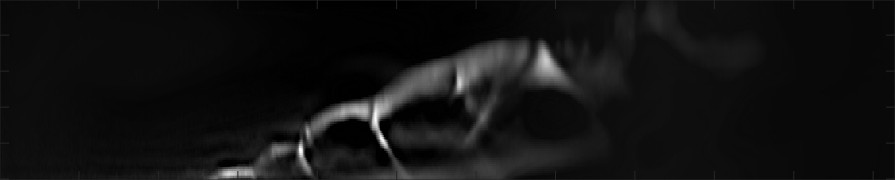
\includegraphics[width=0.5\textwidth]{img/urec_xz1.png}
    \end{minipage}

    \begin{center}
      \mycaption{
        Data (top), constant PSF deconvolution (middle),
        model deconvolution (bottom)
      }
    \end{center}



    
%    \begin{minipage}[h]{\textwidth}
%      Examples of $k=25$ sources in an image with $67 \times 67$ 
%      pixels (giving $m=4489$ measurements), Gaussian kernel
%      with $\sigma = 0.05$ and level method parameters
%      $\Pi = 100$ and $B = 100$.
%      Red crosses 
%        
\includegraphics[height=0.007\textheight]{img/cross.png}
%       are true sources and 
%      black circles 
%        
\includegraphics[height=0.007\textheight]{img/circle.png}
%       are estimated sources.
%      
%     \vspace{0.7em}
%      \begin{minipage}[t]{0.49\textwidth}
%        \centering
%        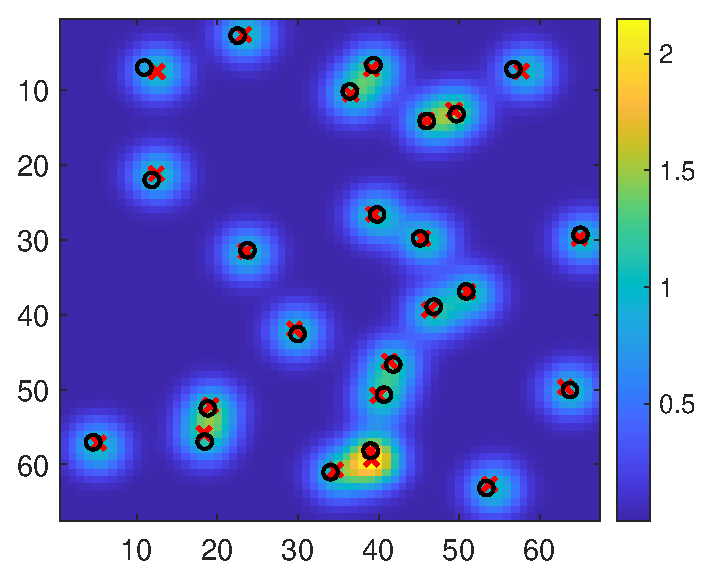
\includegraphics[height=0.1\textheight]{img/2d_noise_free_nolegend.eps}
%
%        \vspace{-0.3em}
%        \mycaption{
%          Noise-free measurements.
%        }
%      \end{minipage}
%      %
%      \begin{minipage}[t]{0.49\textwidth}
%        \centering
%        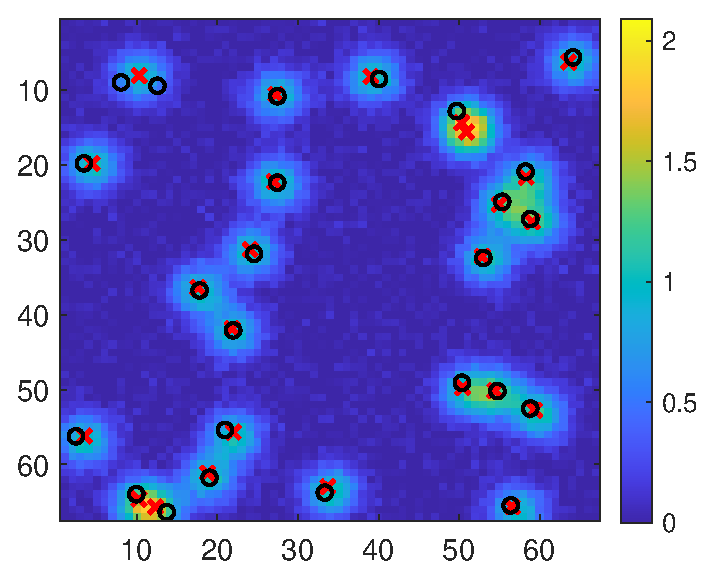
\includegraphics[height=0.1\textheight]{img/2d_noise_005_nolegend.eps}
%
%        \vspace{-0.3em}
%        \mycaption{
%          Gaussian noise with standard deviation $0.05$.
%        }
%      \end{minipage}
%
%      \vspace{0.9em}
%      \begin{minipage}[t]{0.49\textwidth}
%        \centering
%        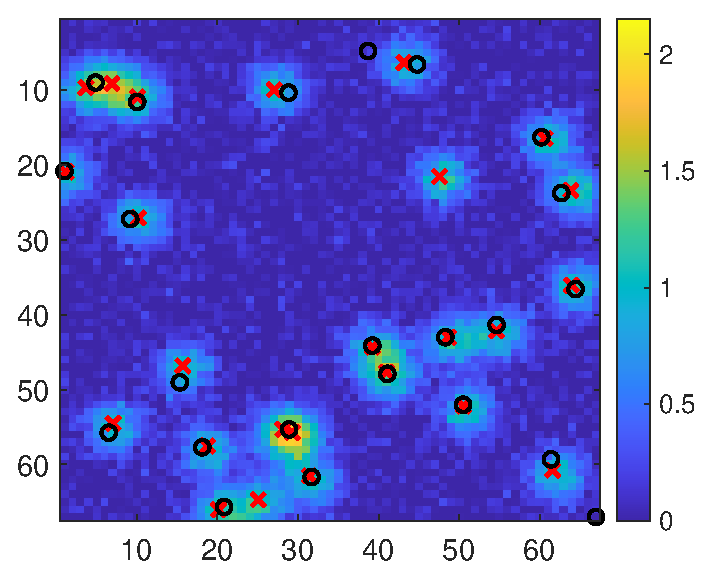
\includegraphics[height=0.1\textheight]{img/2d_noise_01_nolegend.eps}
%
%        \vspace{-0.3em}
%        \mycaption{
%          Gaussian noise with standard deviation $0.1$.
%        }
%      \end{minipage}
%      %
%      \begin{minipage}[t]{0.49\textwidth}
%        \centering
%        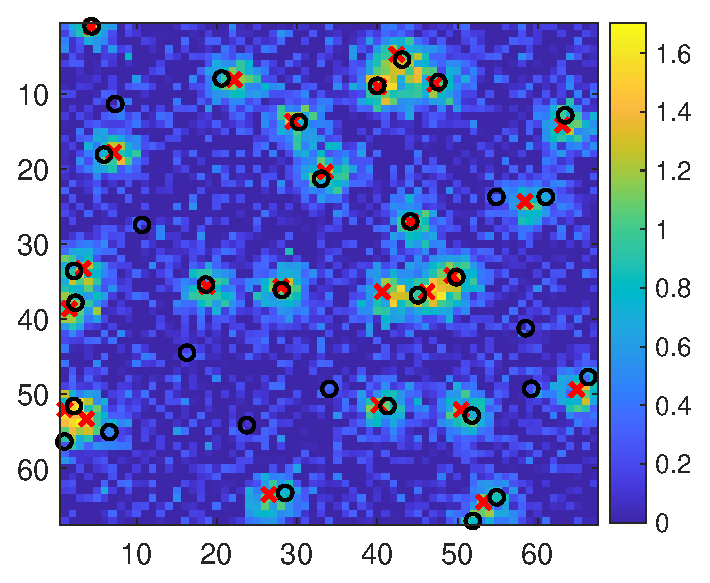
\includegraphics[height=0.1\textheight]{img/2d_noise_02_nolegend.eps}
%
%        \vspace{-0.3em}
%        \mycaption{
%          Gaussian noise with standard deviation $0.2$.
%        }
%      \end{minipage}
%    \end{minipage}
  \end{minipage}
  \vspace{-1em}
}

\headerbox{References}
{name=references, column=0,  below=resultsreal, span=3}
%{name=references, column=0,  above=bottom, span=1}
{
  %\smaller                                  % Make the whole text smaller
  %\footnotesize
  %\scriptsize
  \tiny
  \bibliographystyle{abbrv}                 % Use plain style
  \renewcommand{\section}[2]{\vspace{0.05em}}	% Omit "References" title
  \bibliography{references}
}

\headerbox{Acknowledgments}
{name=acknowledgments, column=3, below=resultsreal, span=3}
%{name=acknowledgments, column=1, above=bottom, span=1}
{  
  \scriptsize
  %\tiny
  This work is funded by 
  Isaac Newton Trust/Wellcome Trust ISSF/University of Cambridge 
  Joint Research Grants Scheme, RG89305.
%  \vspace{-0.6em}
%  \begin{center}
%    \begin{tabular}{cccc}
%      
\includegraphics[height=0.02\textheight]{./img/epsrc_logo.eps}
%      &
%      
\includegraphics[height=0.018\textheight]{./img/InFoMM}
%      &
%      
\includegraphics[height=0.02\textheight]{./img/company_logo.jpg}
%      &
%      
\includegraphics[height=0.018\textheight]{./img/turinglogo2.jpg}
%    \end{tabular}
%  \end{center}
  \par
}






\end{poster}
\end{document}

%%% Local Variables:
%%% mode: latex
%%% TeX-master: t
%%% End:
